\documentclass[twoside, 10pt]{article}

\usepackage{geometry}
\geometry{outer=3em, inner=2.2cm, top=6em, bottom=4em, headheight=\paperheight}
\usepackage[export]{adjustbox}
\usepackage{array}
\usepackage{amsmath}
\usepackage{amsfonts}
\usepackage{fancyhdr}
\pagestyle{fancy}
\fancyhf{}
\lhead{Algebra II - BASE}
\chead{Function Compositions}
\rhead{AO Test, Page \thepage}
\usepackage{lastpage}
\usepackage{xcolor}
\usepackage{enumitem}
\usepackage{pifont}
\usepackage{graphicx}
\graphicspath{{../img}}
\usepackage{pgfplots}
\pgfplotsset{compat=1.18}
\usepackage{tabularx}
\usepackage{tikz}
\usetikzlibrary{patterns}

\newcommand{\R}{\mathbb R}
\newcommand{\e}{{\rm e}}
\newcommand{\pobr}[1]{\left\langle#1\right\rangle}
\newcommand{\norm}[1]{\lVert #1 \rVert}
\newcommand{\abs}[1]{\lvert #1 \rvert}

\DeclareMathOperator{\xd}{d\!}
\DeclareMathOperator{\proj}{proj}

\title{}
\date{}

\begin{document}
\noindent
{\large
First Name \rule{6em}{.1pt}\hspace{\stretch{1}}Last Name \rule{6em}{.1pt}\hspace{\stretch{1}} Date \rule{1.5em}{.1pt} -- \rule{1.5em}{.1pt} -- \rule{1.5em}{.1pt}\hspace{\stretch{1}} Period \rule{2em}{.1pt}\hspace{\stretch{1}} Score \rule{2em}{.1pt}
}
\vspace{1em}

\begingroup
\renewcommand{\arraystretch}{1.5}
\begin{center}
\tiny
{
\begin{tabularx}{\textwidth}{|X|X|X|X|X|X|}
\hline
\bf BE PRECISE & \centerline{Integrating} & \centerline{Applying} & \centerline{Practicing} & \centerline{Acquiring} & \centerline{Awaiting Evidence} \\
\hline
I can calculate accurately and efficiently, and be precise in all of my math.&
Selects and applies the correct procedure and solves all routine AND integrating problems.

AND

Expresses the answer to the correct level of precision needed for the problem (including the correct rounding, units, math symbols, labeling, graphing, vocab…)
&Selects and applies the correct procedure and solves all routine problems.


AND

Expresses the answer to the correct level of precision needed for the problem (including the correct rounding, units, math symbols, labeling, graphing, vocab…)
&Selects and applies the correct procedure and solves most routine problems.


AND

Expresses the answer to the correct level of precision needed for the problem (including the correct rounding, units, math symbols, labeling, graphing, vocab…)
&Selects and applies the correct procedure and solves some routine problems.


AND

Attempts to express the answer to the correct level of precision needed for the problem (including the correct rounding, units, math symbols, labeling, graphing, vocab…).
&Selects and attempts to apply the correct procedure for some routine problems.\\
\hline
\bf Criteria&\multicolumn{5}{l|}{\parbox[c][4em]{.8\textwidth}{}}\\
\hline
\end{tabularx}
}
\end{center}
\endgroup

\begin{enumerate}
\item
\noindent
{\bf Survey.} If there is a ``distraction-free zone'' in the classroom, would you like to reserve a seat in it, knowing that residents of this zone agree to follow the distraction-free policy?\hspace{2em}{\bf Yes}\hspace{3em}{\bf No}

{\it (Note: You will receive a 0.5 point deduction for not answering this survey question.)}
\item
The standard form of a quadratic equation is $ax^2 + bx + c = 0$.
Identify the $a$, $b$ and $c$ for the following equations:
\begin{enumerate}[label=(\arabic*)]
\item $2x^2 - 5x + 2 = 0$.\hspace{2em}
$
a = \rule{5em}{.1pt}\ b=\rule{5em}{.1pt}\ c = \rule{5em}{.1pt}
$\\

\item $-5x^2 + 3x  + 23 = -44$.\hspace{2em}
$
a = \rule{5em}{.1pt}\ b=\rule{5em}{.1pt}\ c = \rule{5em}{.1pt}
$

\end{enumerate}

\item Let $f(x)=3x+2$ and $g(x) = x^2$. 
\begin{enumerate}
\item
Find $f(g(-3))$.
\vspace{\stretch{1}}
\item
Find $g(x+1)$ and simplify.
\vspace{\stretch{1}}
\item
Find $(g\circ f)(x)$ and simplify.
\vspace{\stretch{1}}
\end{enumerate}
\item
\begin{tabular}{cc}
\begin{tabular}{|c|c|c|c|c|c|c|}
\hline
x&1.0&1.5&2.0&2.5&3.0&3.5\\
\hline
f(x)&2.8&2.6&2.5&2.0&1.0&2.2\\
\hline
\end{tabular}\hspace{.1\textwidth}
&
\begin{tabular}{|c|c|c|c|c|c|c|}
\hline
x&2.0&2.2&2.4&2.6&2.8&3.0\\
\hline
g(x)&1.2&1.5&3.0&2.8&2.5&2.0\\
\hline
\end{tabular}
\end{tabular}

Find the following using the tables above:
\begin{enumerate}
\item
$(g\circ f)(1.0)$
\vspace{\stretch{1}}
\item
$(f\circ g)(2.2)$
\vspace{\stretch{1}}
\item
$(g\circ g)(3.0)$
\vspace{\stretch{1}}
\end{enumerate}
\clearpage

\item
The graph below contains the lines for $h(x)$ and $k(x)$. Use it to find the following:

\begin{tabular}{ll}
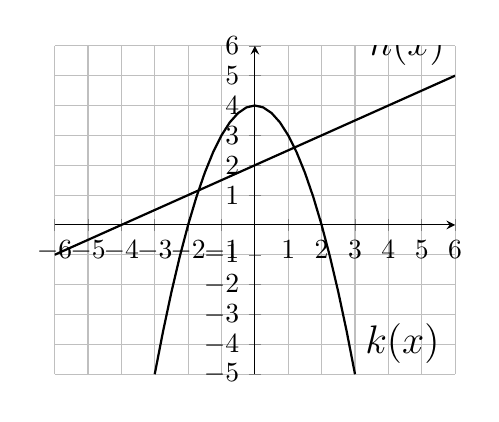
\begin{tikzpicture}[baseline=(current bounding box).middle]
\begin{axis}[
axis lines=middle,
grid=both,
xtick distance=1,
ytick distance =1,
ymin=-5, ymax=6,
xmin=-6, xmax=6,
width = 0.55\textwidth
]
\addplot[thick, domain=-3:3]{-(x^2 - 4)} node[pos=1, above right]{\Large $k(x)$};
\addplot[thick, domain=-6:6]{1/2*x + 2} node[pos=1, above left]{\Large $h(x)$};
\end{axis}
\end{tikzpicture}\hspace{.1\textwidth} &\parbox{.4\textwidth}{
\begin{enumerate}[label=\alph*)]
\item $(h\circ k)(3) = $\\[2em]
\item $(h\circ k)(2) = $\\[2em]
\item $(k \circ h)(-2) =  $\\[2em]
\item $(k\circ h)(-4) = $
\end{enumerate}}
\end{tabular}

\item When a small stone is dropped into a calm pond, the radius of the outermost visible ripple (in centimeters) after $t$ seconds is modeled by 
\[
r(t) = 6\sqrt{t}.
\]
The area of the ripple (in cm$^2$) is given by $A(x) = \pi x^2$. 
Assume the ripple fades and disappears after $10$ seconds.

\begin{enumerate}[label=(\alph*)]
\item Find $(A\circ r)(t)$ and simplify.
\vspace{\stretch{1}}
\item Find the realistic domain and range of $(A\circ r)(t)$.
\vspace{\stretch{1}}
\item Explain in words what $(A\circ r)(t)$ represents in this situation.
\vspace{\stretch{1}}
\end{enumerate}
\end{enumerate}

\end{document}